% Created 2018-10-14 Sun 14:58
% Intended LaTeX compiler: pdflatex
\documentclass[11pt]{article}
\usepackage[utf8]{inputenc}
\usepackage[T1]{fontenc}
\usepackage{graphicx}
\usepackage{grffile}
\usepackage{longtable}
\usepackage{wrapfig}
\usepackage{rotating}
\usepackage[normalem]{ulem}
\usepackage{amsmath}
\usepackage{textcomp}
\usepackage{amssymb}
\usepackage{capt-of}
\usepackage{hyperref}
\date{\today}
\title{A Critical Analysis of Experimental and Theoretical Assumptions Involved in Manometric Adsorption Characterization of Gas Shales and their Net Effects on Reserve Estimation and Production Forecasts}
\hypersetup{
 pdfauthor={},
 pdftitle={A Critical Analysis of Experimental and Theoretical Assumptions Involved in Manometric Adsorption Characterization of Gas Shales and their Net Effects on Reserve Estimation and Production Forecasts},
 pdfkeywords={},
 pdfsubject={},
 pdfcreator={Emacs 26.1 (Org mode 9.1.13)}, 
 pdflang={English}}
\begin{document}

\maketitle
\tableofcontents


\section{Abstract}
\label{sec:orgec58a62}
\section{Introduction}
\label{sec:org1ab1a49}
\begin{itemize}
\item gas shale reservoirs have been enjoying increasing amounts of attention from the industry and academia as a promising low-carbon energy source for the 21st century
\item it is now well known that sorption phenomena play a significant role in gas storage and production processes from gas shales; nearly 20-80\% of the total gas in gas shales is stored in the adsorbed state \cite{schettlerjr1991}
\item that said, the lack of reproducibility of adsorption isotherms measured in different laboratories is a significant roadblock to shale reservoir characterization
\item whilst we concede that the highly heterogeneous nature of shales are at least partly responsible for this, significant improvements to experimental reporducibility could be made through diligent control and reporting of experimental parameters
\item this study will review our current understanding of manometric adsorption characterization of shales, and provide a critical analysis on the effect of the assumptions involved in the process on reservoir characterization, through an one dimensional reservoir simulation
\end{itemize}
\section{Methodology}
\label{sec:org23c0221}
\subsection{Sample description}
\label{sec:org47727f2}
\begin{itemize}
\item for this study, shale outcrop samples from the oil shale mine in straiton are used
\item outcrop samples were crushed to 350 to 2000 \(\mu\) m and stored in air-tight containers under dark until the start of experiment
\end{itemize}
\subsection{Adsorption and diffusion characterization}
\label{sec:org249ffdc}
\begin{itemize}
\item analysis methodology, adopted after \cite{rouquerol1994}, is outlined below
\end{itemize}
\begin{center}
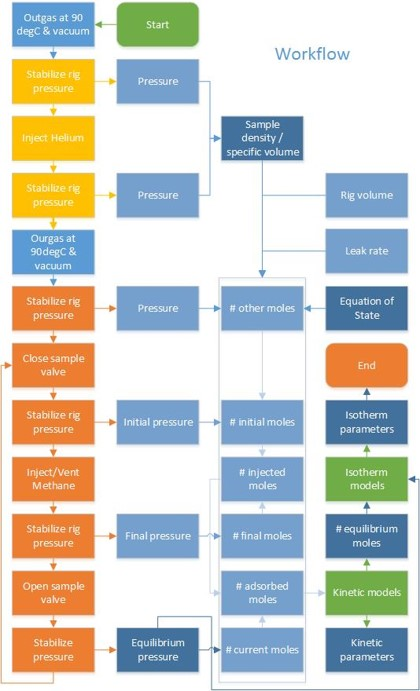
\includegraphics[width=.9\linewidth]{./adsorption_workflow.jpg}
\end{center}
\begin{itemize}
\item samples were loaded on to the adsorption rig, and the rig was flushed with Helium several times to remove any residual gas from previous experiments
\item samples were then outgassed in-situ at 90 degC and 150 Torr pressure
\item after outgassing the rig was brought down to experimental temperature and allowed to reach equilibrium at about 500 Torr pressure
\item performing outgassing in-situ in an inert near-vacuum atmosphere allows us to minimize any exposure to air, moisture, or any other adsorptive that might otherwise affect our measurements
\item adsoprtion and desorption was measured through a step-wise procedure as outlined in the diagram
\item the reference and sample cells are isolated; adsorptive is injected into the reference cell and allowed to reach thermal equilibrium; the sample valve is then opened and the rig pressure was monitored for 2 hours or until equilibrium conditions were met, whichever was longer
\item initial \# moles in the sample cell is using an appropriate Equation of State
\end{itemize}
\begin{equation}
n_{is} = EOS(P_{s},V_{v},T_{s})
\end{equation}
\begin{itemize}
\item where
\begin{itemize}
\item \(n_{is}\) is number of moles initially present in the sample cell before experiment
\item EOS is a function denoting the chosen Equation of State
\item \(P_s\) is sample cell pressure
\item \(V_v\) is sample cell void volume
\item \(T_s\) is sample cell temperature
\end{itemize}
\item sample cell void volume is calculated as
\end{itemize}
\begin{equation}
V_v = V_s - V_{sp} * w_{sh}
\end{equation}
\begin{itemize}
\item where
\begin{itemize}
\item \(V_v\) is sample cell void volume
\item \(V_s\) is sample cell volume
\item \(V_{sp}\) is sample specific volume
\item \(w_{sh}\) is sample weight
\end{itemize}
\item injected \# moles is calculated as
\end{itemize}
\begin{equation}
n_{ir} = EOS(P_{r,f},V_r,T_r) - EOS(P_{r,i},V_r,T_r)
\end{equation}
\begin{itemize}
\item where
\begin{itemize}
\item \(n_{ir}\) is number of moles injected
\item EOS is a function denoting the chosen Equation of State
\item \(P_{r,f}\) is final pressure of reference cell
\item \(P_{r,i}\) is initial pressure of reference cell
\item \(V_r\) is reference cell volume
\item \(T_r\) is reference cell temperature
\end{itemize}
\item \# moles present at any given instance is calculated as
\end{itemize}
\begin{equation}
n_{c} = EOS(P_s,V_r,V_v,T_s)
\end{equation}
\begin{itemize}
\item \(n_{c}\) is number of moles injected
\item EOS is a function denoting the chosen Equation of State
\item \(P_{s}\) is final pressure of reference cell
\item \(P_{s}\) is initial pressure of reference cell
\item \(V_r\) is reference cell volume
\item \(V_v\) is sample cell volume
\item \(T_s\) is sample cell temperature
\end{itemize}
\begin{itemize}
\item excess adsobed \# moles for the nth pressure step is calculated as
\end{itemize}
\begin{equation}
n_{e} = n_{ir}(1) + n_{ir}(2) + \dots + n_{ir}(n) + n_{is} - n_c
\end{equation}
\begin{itemize}
\item where
\begin{itemize}
\item \(n_{ir}(n)\) is amount of moles injected at nth pressure step
\item various assumptions involved in the calculation of amount adsorbed are discussed in more detail below
\end{itemize}
\end{itemize}
\subsubsection{Gibbs Approach}
\label{sec:org10690e8}
\begin{enumerate}
\item Gas Phase Concentration Correction Term
\label{sec:org2777d63}
\begin{itemize}
\item amount adsorbed is defined as the number of adsorptive molecules distributed in the adsorption space
\item adsorption measurement rigs, on the other hand, in effect measure the difference in distribution of the adsorptive molecules in the gas phase and the adsorption space, between the initial and final states of the experiment to calculate amount adsorbed - this is defined to be the Gibbs excess sorption \cite{Rouquerol2016}
\item as some gas molecules are distributed in the adsorption space both in the initial and final states, excess sorption values under estimate the actual amount of adsorptive molecules present in the adsorption space
\item the molar density of the gas phase being reasonably small in low pressures, this error is usually negligible
\item at pressures greater than 10 MPa, however, this error becomes significant and must be accounted for
\item experimentally observed excess sorption values - difference in the distribution of adsorptive molecules between the initial and final states - maybe corrected to absolute sorption values - amount af adsorptive molecules distributed in the adsorption space, either by assuming that the adsorbed phase density remains constant with loading, or that the adsorption space (volume of the adsorbed phase) remains constant with loading
\item constant adsorbed density
\end{itemize}
\begin{equation}
n_{a} = \frac{n_{e}}{1-\frac{\rho_{g}}{\rho_{ads}}}
\end{equation}
\begin{itemize}
\item constant adsorbed volume
\end{itemize}
\begin{equation}
n_{a} = n_{e} + \rho_g * V_{ads}
\end{equation}
\begin{center}
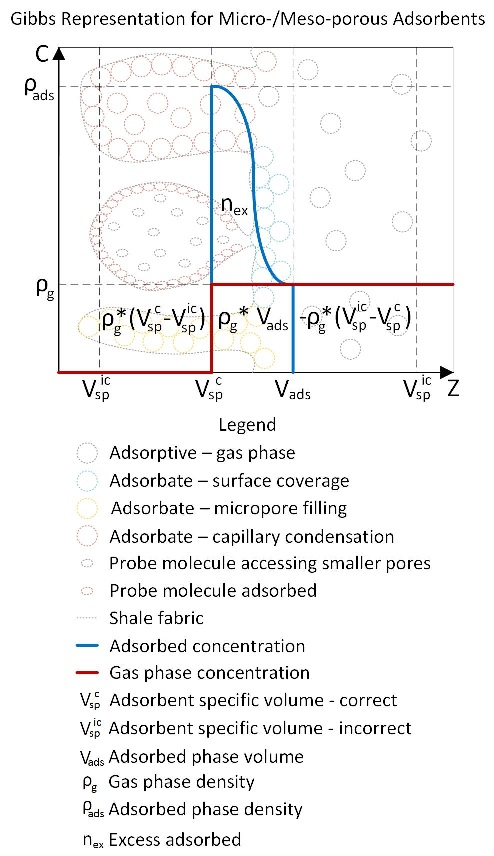
\includegraphics[width=.9\linewidth]{./gibbsrepresentation.jpg}
\end{center}
\item Void Volume Correction Term
\label{sec:orgc9360b9}
\begin{itemize}
\item the previous section discussed correcting experimentally observed excess sorption values - difference in the distribution of adsorptive molecules between the initial and final states - maybe corrected to absolute sorption values - amount af adsorptive molecules distributed in the adsorption space,
\item the definition of adsorption space itself could be problematic in microporous substances
\item discussed in more detail in the \href{bowlandpore.org}{pore characterization paper}
\item accurate characterization of the shale's specific volume can be problematic, and is now recognized as one of the biggest error source in the adsorption characterization of micro-porous substances \cite{Rouquerol2016}
\item all pore characterization metrics are characteristic measures of the methodology employed
\item for the purpose of gas adsorption measurement, therefore, it is preferable to apply an experimental technique that most closely simulates pore characteristics observed during methane adsorption on gas shales
\item ideally this technique would involve calibration of a shale's specific volume using a non-adsorbing probe molecule of a similar size to the adsorptive, however this can seldom be achieved in the laboratory
\item errors induced in void volume calibration may be due to the probe molecule (usually Helium) being of a different size compared to the adsorptive molecule, and due to the probe molecule being adsorbed under calibration conditions
\item as a compromise, void volume was measured using Helium at three temperatures 30, 60, and 90 degC at about 500 Torr pressure; the van der Waals equation of state was used for this purpose
\item the reason for measuring specific volume in these conditions is to
\item some authors \cite{Rouquerol2016}, \cite{Brandani2017}, \cite{Pini2014} propose using a using a specific volume of 0.5 cc/g, corresponding to a density of 2 kg/m3; however this arbitrarily defined adsorbate specific volume might be too high for gas shales whose reported densities usually range between 2.4 to 2.8 kg/m3, corresponding to specific volume values between 0.36 and 0.42 cc/g
\item amount adsorbed may be corrected for incorrectly measured specific volumes as follows
\end{itemize}
\begin{equation}
n ^{c} = n ^{ic} + \rho _g ( V _{sp} ^{c} - V _{sp} ^{ic} )
\end{equation}
\end{enumerate}
\subsubsection{Other Assumptions}
\label{sec:org97a256f}
\begin{enumerate}
\item Equation of State
\label{sec:orgae3e73c}
\begin{itemize}
\item various Equations of State were considered for the calculations described above
\item ideal
\end{itemize}
\begin{equation}
PV = nRT
\end{equation}
\begin{itemize}
\item van der Waals
\end{itemize}
\begin{equation}
(P + \frac{an^2}{V^2})(V-nb) = nRT
\end{equation}
\begin{itemize}
\item cubic equations of state
\end{itemize}
\begin{equation}
P = \frac{RT}{V-b} - \frac{a(T)}{(V+\epsilon b)(V+\sigma b)}
\end{equation}
\begin{itemize}
\item the Peng-Robinson and Redlich-Kwong cubic equations of states were used for this study
\item fitting parameters: \(\epsilon\), \(\sigma\), a(T), and b were obtained from \cite{Perry1950}
\item all equations of state were solved using an iterative procedure with an initial estimate obtained from the ideal gas law, until an accuracy of 1e-6\% was achieved
\end{itemize}
\item Equilibrium Adsorption Rate
\label{sec:orgd9ab0d9}
\begin{itemize}
\item the adsorption profile over time was fitted using a rolling regression with a window of 100 readings (\textasciitilde{}30 minutes)
\item equilibrium was assumed when the rate of sorption (slope of the regression line) fell below 5e-8 mmol/g (mol/kg)
\end{itemize}
\item Leak Rate
\label{sec:org17226bb}
\begin{itemize}
\item home-made high pressure adsorption rigs usually have a small leak
\item due to the long equilibrium times required for shale adsorption, even small leaks may have a significant effect in adorption calculations; these must be accounted for
\item several studies have incorrectly assumed a constant leak rate for all adsorption steps
\item leak rates maybe characterized as a flow through an orifice using the Poiseuille's law for gaseous flow \cite{Bomelburg1977}
\end{itemize}
\begin{equation}
Q = \frac{\pi R^4 (P_1 ^2 - P_2 ^2)}{16 \eta l P_2}
\end{equation}
\begin{itemize}
\item Q is the volumetric flow of the outlet side pressure (atmospheric pressure)
\item \(P_1\) is the rig pressure
\item \(P_2\) is atmospheric pressure
\item R is radius of opening
\item l is length of opening
\item \(\eta\) is the viscosity of the fluid
\item hence it's sufficient to measure leak resistance at one sufficiently high pressure, to be able to account for it for the entire adsorption isotherm
\item it was noted that leak rates were not constant with time - they varied between various experiments based on the efficiency of the compression fittings used
\end{itemize}
\end{enumerate}
\subsubsection{Adsorption Models}
\label{sec:org4d9301b}
\begin{itemize}
\item adsorption isotherms are futher analysed and integrated with reservoir simulators through adsorption isotherms
\item to maintain comparable computational demands, all isotherms considered here have only 2 parameters, and result in a Type 1 adsorption isotherm \cite{Sing1985}
\end{itemize}
\begin{enumerate}
\item Langmuir Model
\label{sec:org2c7835f}
\begin{itemize}
\item the most commonly used model to fit adsorption isotherms - the Langmuir theory assumes an energetically homogeneous ideal surface with periodic energy fluctuations larger than the thermal energy of the adsorptive molecule, with the troughs acting as localised adsorption sites that can accommodate a single adsorptive molecule \cite{Langmuir1918}
\end{itemize}
\begin{equation}
n_{ads} = \frac{V_L*P}{P_L + P}
\end{equation}
\begin{itemize}
\item \(n_{ads}\) is amount adsorbed
\item \(V_L\) is the Langmuir volume
\item P is the pressure
\item \(P_L\) is the Langmuir pressure
\end{itemize}
\item Potential Model
\label{sec:orgd27d739}
\begin{itemize}
\item was proposed by \cite{Dubinin1960} for subcritical vapours in microporous solids
\item amount adsorbed can be expressed in terms of adsorption potential, independent of temperature as follows
\end{itemize}
\begin{equation}
\frac{V}{V_0} = - B A ^2
\end{equation}
\begin{equation}
V = V_0 exp[-\frac{1}{E} (R T ln (\frac{P}{P_0}))^2]
\end{equation}
\begin{itemize}
\item E0 is the characteristic energy of the solid toward an arbitrarily chosen reference adsorbate; Benzene is widely used as the reference adsorbate
\item maximum adsorption capacity is given as
\end{itemize}
\begin{equation}
V_0 = \frac{W_0}{v_M(T)}
\end{equation}
\begin{itemize}
\item \(W_0\) is the micropore volume
\item \(v_m\) is the liquid molar volume
\item the DR model often provides a better fit for shale adsorption, despite having the same number of parameters as Lanmmuir \cite{Clarkson1997}
\end{itemize}
\item Freundlich Model
\label{sec:org38da783}
\begin{itemize}
\item initially proposed as an empirical approach, the Freundlich model, can also be derived theoretically based on an adsorption potential approach by assuming an heterogeneous surface with independent patches, whose energy distribution follows an exponential decay function, and that adsorption in each individual patch follows the Langmuir theory \cite{Do1998}
\item since adsorption sites in shales are highly heterogeneous, the Freundlich model may be particularly well suited to model gas adsorption in shales.
\item one of the main drawbacks of the Freundlich model is that it does not have proper Henry's law behavior, or a finite limit at sufficiently high pressures, the model can only be applied to a narrow pressure range, although this is usually sufficient for the purpose of reservoir simulations
\end{itemize}
\begin{equation}
q = K * P ^{1/n}
\end{equation}
\begin{itemize}
\item K and n are fitting parameters
\item parameter n is usually greater than 1 and increases with increasing heterogeneity
\end{itemize}
\item Isosteric Heat of Adsorption
\label{sec:orgc8b7e07}
\begin{itemize}
\item the isosteric heat of adsorption is commonly used to compare energetics of adsorption between different adsorbate-adsorptive combinations
\item the isosteric heat of adsorption at a given amount adsorbed is calculated by solving the differential of the isotherm with respect to temperature at fixed surface coverage and the \href{vanthoffequation.org}{van't Hoff equation}
\end{itemize}
\begin{equation}
(\frac{d ln P}{d \frac{1}{T}})_{n} = -\frac{\Delta H}{R}
\end{equation}
\begin{itemize}
\item isosteric heat was calculated based on the regression slope between ln P and 1/T at given amount adsorbed for isotherms at different temperature
\item however for the purpose of reservoir simulation, it is more convenient to use temperature dependence relations of concerned isotherm parameters listed in previous secions
\end{itemize}
\end{enumerate}
\subsubsection{Diffusion Models}
\label{sec:orgcf39d48}
\begin{itemize}
\item adsorption and diffusion kinetics can either be modelled with a lumped parameter model, using a kinetics approach, or with a distributed parameter model, based on the diffusion equation
\end{itemize}
\begin{enumerate}
\item First Order
\label{sec:org9de5b51}
\begin{itemize}
\item initially proposed by \cite{Lagergren1898}, this is the earliest model pertaining to adsorption rate based on adsorption capacity
\item rate of adsorption is assumed to be directly proportional to the driving force (concentration difference), with the first order diffusion constant as the proportionality constant
\end{itemize}
\begin{equation}
\frac{dq_}{dt} = k_1 * (q_e - q)
\end{equation}
\begin{itemize}
\item this can be integrated by simply separating the variables
\item an incorrect initial condition of \(q(0)= 0\) is usually assumed in the literature, whilst adopting a procedure after \cite{Rouquerol2013}, where initial adsorption is not 0 for all pressure steps except the first
\item therefore we propose the following boundary conditions for integration \(q(0) = q_0\) and \(q(t) = q_t\), yeilding the following relation
\end{itemize}
\begin{equation}
q_t = q_e - q_e exp(-k_1 t) + q_0 exp(-k_1 t)
\end{equation}
\item Second Order
\label{sec:org21d15f5}
\begin{itemize}
\item second order sorption kinetics, theoretically based on chemisorption on bi-valent sorbates \cite{Fan2003a}, \cite{Qiu2009}, maybe empirically applied to shales
\end{itemize}
\begin{equation}
\frac{dq}{dt} = k_2 * (q_e - q)^2
\end{equation}
\begin{itemize}
\item integrating by separating variables between \(q(0) = q_0\) and \(q(t) = q_t\):
\end{itemize}
\begin{equation}
q_t = \frac{q_e k_2 t |q_e - q_0| + q_0}{1 + k_2 t |q_e - q_0|}
\end{equation}
\begin{itemize}
\item q\(_{\text{t}}\) is amount adsorbed at time t
\item k\(_{\text{2}}\) is pseudo second order rate constant
\item q\(_{\text{e}}\) is amount adsorbed at equilibrium
\item q\(_{\text{0}}\) is amount adsorbed at time 0
\end{itemize}
\item Elovich Model
\label{sec:org5fc899f}
\begin{itemize}
\item initially proposed for chemisorption in heterogeneous solids \cite{Qiu2009}, the Elovich model assumes that rate of sorption decreases with the exponential of surface coverage
\end{itemize}
\begin{equation}
\frac{dq}{dt} = a * e ^{-\alpha q}
\end{equation}
\begin{itemize}
\item q is amount adsorbed
\item a is desorption constant that determines equilibrium sorption rate
\item \(\alpha\) is initial adsorption rate, which is negative for desorption
\end{itemize}
\begin{itemize}
\item integrating between \(q(0) = q_0\) and \(q(t) = q_t\)
\end{itemize}
\begin{equation}
q_t = \frac{log(| exp(\alpha q_0) + a t / \alpha |)}{\alpha}
\end{equation}  
\item Fick's Laws
\label{sec:org6cc4b7c}
\begin{itemize}
\item the Diffusion equation is given as \cite{Crank1979}
\end{itemize}
\begin{equation}
\frac{\partial C}{\partial t} = \nabla (D . \nabla C)
\end{equation}
\begin{itemize}
\item for isotropic media it takes the same form as the heat equation
\end{itemize}
\begin{equation}
\frac{\partial C}{\partial t} = D (\nabla^2 C)
\end{equation}
\begin{itemize}
\item for cylindrical co-ordinates
\end{itemize}
\begin{equation}
\frac{\partial C}{\partial t} = 
D * \frac{\partial^2 C}{\partial r^2} = 
D (\frac{\partial ^2 C}{\partial z ^2} + 
\frac{1}{A} + \frac{\partial A}{\partial z} \frac{\partial C}{\partial z})
\end{equation}
\item Weber Morris
\label{sec:orgde50286}
\end{enumerate}
\subsubsection{Shale Reservoir Model}
\label{sec:org279b57a}

\subsection{Standard Assumptions}
\label{sec:org1fb8021}
\begin{itemize}
\item in order to facilitate comparison between different
\end{itemize}
\begin{center}
\begin{tabular}{ll}
Parameter & Measurement conditions / assumptions\\
Shale specific volume & Measured at 90 degC 500 Torr pressure\\
Gas phase concentration & Constant adsorbed phase volume (micropore filling)\\
Equation of state & van der Waals\\
Equilibrium conditions & < 5e-7 mol over 30 mins\\
Leak rates & Modelled as flow through an orrifice\\
Adsorption model & Langmuir\\
\end{tabular}
\end{center}
\section{Results}
\label{sec:org304d5ea}
\subsection{Specific Volume Correction}
\label{sec:org0636dd9}
\subsection{Gas Phase Concentration Correction}
\label{sec:org31e3297}
\subsection{Equations of States}
\label{sec:orgf2abfb6}
\subsection{Equilibrium Conditions}
\label{sec:orgaf6d6ad}
\subsection{Leak Rates}
\label{sec:org15f6f56}
\subsection{Adsorption Models}
\label{sec:org837c5fe}
\subsection{Diffusion Models}
\label{sec:orgb8e4be9}
\section{Discussions}
\label{sec:orgfa9443c}
\subsection{Gibbs Approach}
\label{sec:org1b3f61e}
\subsubsection{Specific Volume Correction Term}
\label{sec:org068e80b}
\subsubsection{Gas Phase Concentration Correction Term}
\label{sec:orgddb3c11}
\subsection{Other Assumptions}
\label{sec:org199b507}
\subsubsection{Equation of State}
\label{sec:orga196d77}
\begin{itemize}
\item ideal gas law under-estimates sorption by nearly 10\% compared to van der Waals equation of state
\item it can also be seen that the desorption curve falls below the adsorption curve in many cases when ideal gas law is used - indicating that real gas laws need to be used to fit high pressure adsorption isotherms
\item when real gas law with compressibility factors from NIST REFPROP is used, there is very little to no hysteresis compared to van der Waals equation of state
\end{itemize}
\subsubsection{Equilibrium Adsorption Rate}
\label{sec:org57465fb}
\begin{itemize}
\item it was noted that most of the sorption occured within a few fractions of a seconds
\item the adsorption profile over time was fitted using a rolling regression with a window of 200 readings (\textasciitilde{}30 minutes)
\item equilibrium was assumed when the rate of sorption (slope of the regression line) fell below 5e-8 mmol/g (mol/kg)
\item as seen from the figure, most of the adsorption occurs instantaneously
\item however, sorption can be seen to proceed at a much slower rate (<5e-7) for extended periods of time
\item this phenomenon is particularly pronounced in highly organic and microporous samples
\item equilibrium conditions donot significantly affect the isotherm except in highly organic and microporous adsorbates
\end{itemize}
\subsubsection{Leak Rate}
\label{sec:org10780c9}
\subsection{Adsorption Models}
\label{sec:org6823f77}
\subsection{Kinetic Models}
\label{sec:org883a50f}
\end{document}
